\chapter{\textbf{Cloud infrastructure management}}


This section will be used to described OpenNebula, that is a virtual infrastructure (VI) manager. Organizations can use it to manage and deploy VMs, individually or in groups that must be co-scheduled on local or external resources, which means that it supports hybrid clouds. Some of its key features are:
\begin{itemize}
 \item It provides a homogeneous view of resources, regardless of the underlying hypervisor (e.g. KVM, Xen). This makes the virtualization much less restrictive. The physical machine in which the VM is being run does not need to be tied to a specific virtualization technology, causing incompatibility issues;
  \item Manage a VM's full life cycle, like managing storage requirements and setting up the network;
  \item Supports configurable resource allocation policy.
\end{itemize}

The OpenNebula architecture is illustrated by ~\ref{fig:open_arch}. Each component is specialized in one aspect of VI management. The core takes care of the VM's life cycle. It has three management areas. The first is the preparation of disk images for the VMs. It needs to control the image and storage technologies. The second area is the setup of the network environment for the VMs . And finally, it needs to control the hypervisors for creating and controlling them. All of these activities are performed through pluggable drivers. This modularity makes the system easier to extend and avoids tying it to any specific technology. Other benefit of the core is the ability to support services	




\begin{figure}[ht]
  \centering
 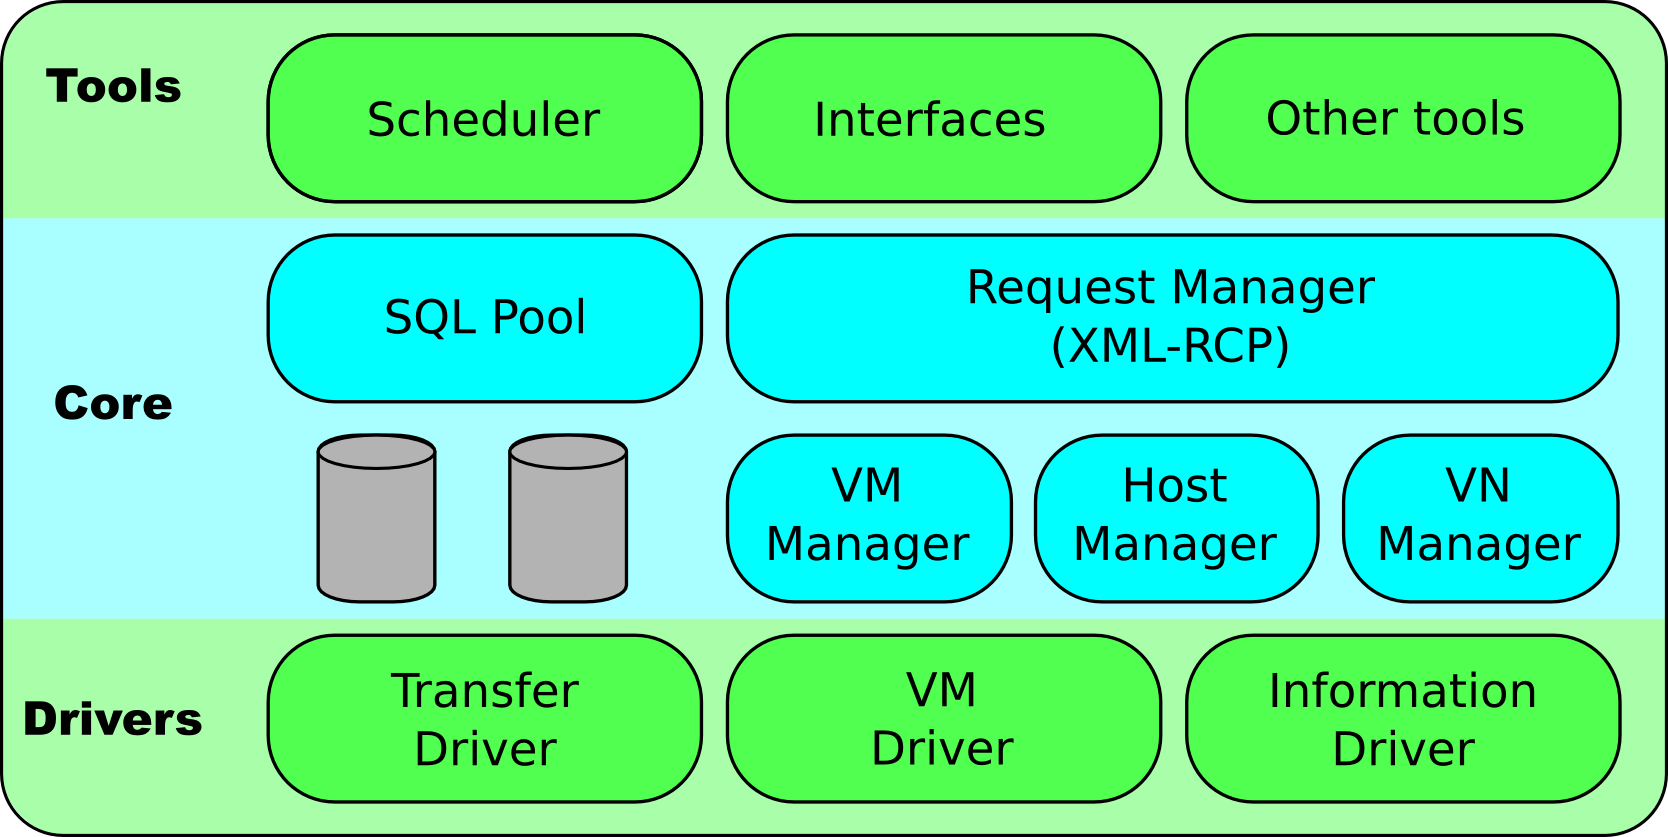
\includegraphics[scale=1]{one-architecture.png}
  \caption{OpenNebula architecture}
  \label{fig:open_arch}
\end{figure}



% However, the scope of this paper is limited to the private part of the cloud, since it's neither possible, nor makes sense to balance the load of an external provider infrastructure.





